\documentclass[a4paper,12pt]{book}

\usepackage[T1]{fontenc}
\usepackage[T2A]{fontenc}
\usepackage[utf8x]{inputenc}
\usepackage[russian]{babel}
\usepackage{geometry}
\usepackage{graphicx}
\usepackage{wrapfig}
\usepackage{caption}

\geometry{left=2.5cm}
\geometry{right=1.5cm}
\geometry{top=0.7cm}
\geometry{bottom=2cm}

\begin{document}
\fontsize{14pt}{14pt}\selectfont
\parindent=0.0cm
{\small 306\ \ \ \ \ \ \ \ \ \ \ \ \ \ \ \ \ \ \ \ \ \ \ \ \ \ \ \ \ \ \ \ \ \ \ \ \ \ \ \ \ \ \ \ \ \ \ \ \ \ \ \ \ \ \ \ \ \ \ $\S$ 20. \textit{Частные производные. Дифференцируемость}
}\par
\vspace{1.5em}
\parindent=0.0cm
\textit{если он существует, называется производной функции $f$ в точке $M_0$ по направлению вектора $\textbf{l}$ и обозначается $\frac{\partial f(M_0)}{\partial l}$}.\par
\parindent=0.7cm
Пусть теперь в пространстве $E^3$ зафиксирована некоторая система координат $x, y, z$. Пусть $M_0 = (x_0, y_0, z_0)$, $M = (x, y, z)$, $\bigtriangleup x = x - x_0$, $\bigtriangleup y = y - y_0$, $\bigtriangleup z = z - z_0$ и $s = M_0M$. Найдем связь между координатами точки $M$ и ориентированной длиной $s$ отрезка $M_0M$.\par
\begin{wrapfigure}{l}{0.5\textwidth}
\vspace{-10pt}
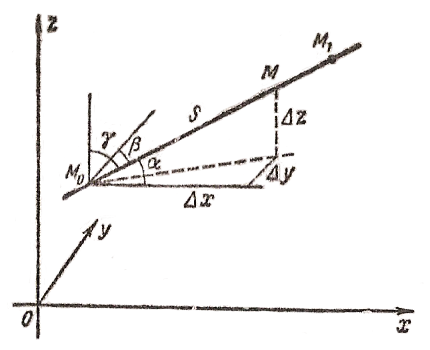
\includegraphics[scale=1.5]{grafik.png}
\begin{center}
\textit{Рис}. 76
\end{center}
\end{wrapfigure}\par
\parindent=0.0cm
Пусть $\alpha$, $\beta$ и $\gamma$ - углы, образованные вектором $\overrightarrow{M_0M_1}$ соответственно с осями $Ox$, $Oy$ и $Oz$. Тогда (рис. 76)\par
$$
x - x_0 = s\cos \alpha,
$$\par
$$
y - y_0 = s\cos \beta,
$$\par
$$
z - z_0 = s\cos \gamma.
$$\par	
\vspace{1.0em}
Вдоль прямой $M_0M$ функция $f$ является функцией одного переменного $s$, а именно\par
\vspace{1.5em}
$$
f(x, y, z) = f(x_0 + s \cos \alpha, y_0 + s \cos \beta, z_0 + s \cos \gamma).
$$\par
\parindent=0.7cm
Производная этой функции по $s$ (если она, конечно, существует) и является \textit{производной функции $f$ в точке $M_0$ по направлению вектора \overrightarrow{M_0M_1}}.\par
Заметим, что направляющие косинусы $\cos \alpha$, $\cos \beta$ и $\cos \gamma$ вектора $\overrightarrow{M_0M_1}$ определяются следующим образом через координаты точек $M_0 = (x_0, y_0, z_0)$ и $M_1 = (x_1, y_1, z_1)$:\par
$$
\cos \alpha = \frac{x_1 - x_0}{p},\quad \cos \beta = \frac{y_1 - y_0}{p},\quad \cos \gamma = \frac{z_1 - z_0}{p}, \eqno{(20.43)}
$$\par
$$
p = \sqrt{(x_1 - x_0)^2 + (y_1 - y_0)^2 + (z_1 - z_0)^2}.
$$\par
Вычисляется производная по направлению по правилу дифференцирования сложной функции. Пусть функция $f(x, y, z)$ дифференцируема в точке $(x_0, y_0, z_0)$ и пусть\par
$$
x = x_0 + s \cos \alpha,\quad y = y_0 + s \cos \beta,\quad z = z_0 + s \cos \gamma. \eqno{(20.44)}
$$\par
Согласно общей формуле для производной сложной функции,\par
$$
\frac{\partial f(M_0)}{ds} = \frac{\partial f(M_0)}{\partial x} \frac{dx}{ds} + \frac{\partial f(M_0)}{\partial y} \frac{dy}{ds} + \frac{\partial f(M_0)}{\partial z} \frac{dz}{ds},
$$\par
\end{document}
